\documentclass[10pt, a4paper]{article}
\usepackage[utf8]{inputenc}
\usepackage[T1]{fontenc}
\usepackage[polish]{babel}
\usepackage[colorlinks = true,
            linkcolor = blue,
            urlcolor  = blue,
            citecolor = blue,
            anchorcolor = blue]{hyperref}
            
\usepackage{amsmath}
\usepackage[table,xcdraw]{xcolor}
\usepackage{subfigure}
\usepackage{float}
\usepackage{graphicx}
\usepackage{pgfplots}
\pgfplotsset{compat=1.17}

\usepackage[sorting=none]{biblatex}
\usepackage{csquotes}
\addbibresource{bibliografia.bib}

\title{[INZ] Notatki}
\author{Adamski Maciej}
\date{Październik 2021}

\begin{document}

\maketitle

\section{Dataset}
\label{section:dataset}
Główny dataset przygotowany do wykorzystania podczas badań i porównania składa się z 80 zdjęć zawierająćych twarze. Źródła zdjęć:

\begin{itemize}
    \item 50 zdjęć wybranych z datasetu \textit{Young and Old Images Dataset} \cite{young_old_dataset}
    \item 30 zdjęć mojego autorstwa
\end{itemize}

Dataset został przygotowany w taki sposób, żeby zawierał zróżnicowane zdjęcia pod wieloma względami, takimi jak: jakość obrazu, oświetlenie, powierzchnia zajmowana przez twarz, kolorystyka, płeć, kolor skóry, częściowe zakrycie twarzy, okulary czy odwrócona w bok głowa. 
Wszystkie 80 zdjęć zostało opisanych przeze mnie na potrzeby badań, w szczególności: obszar twarzy, oczu czy środek źrenic. 
\par
Dodatkowo do badania detekcji źrenic zostanie użyty \textit{MRL Eye Dataset} \cite{mrl_eye_dataset} zawierający zdjęcia oczu wraz z pozycją środka źrenicy.

\section{Detekcja twarzy}

\subsection{Cascading Classifier}

\subsubsection{Haar Cascade}

\subsubsection{LBP Cascade}




\subsection{Deep Neural Network}
Jeden z modułów \textit{OpenCV-contrib} \cite{opencv_contirb}. Służy do ładowania modeli głębokich sieci neuronowych i przepuszczeniu przez nie obrazów (lub ich części) celem wykrycia różnych obiektów.

\subsubsection{Caffemodel}
Jednym z modeli dostępnych do detekcji twarzy przy pomocy głebokich sieci neuronowych są modele Caffe (\textit{Convolutional Architecture for Fast Feature Embedding}) \cite{jia2014caffe}.\\
Aktualnie używany w projekcie wzorzec caffe to \\\textit{res10{\_}300x300{\_}ssd{\_}iter{\_}140000{\_}fp16}.


\subsection{Filtrowanie wyników}
\label{section:face_detection_filter}

Użyte algorytmy mogą dawać w wyniku błędnie określone obszary twarzy. Z tego względu zwróconą tablicę obszarów poddaje filtrowaniu.
\begin{itemize}
    \item Pierwszym etapem jest odrzucenie obszarów, których środek znajduje się poza ustalonym pionowym obszarem (przyjałem przedział [0.25, 0.75] szerokości). Wynika to z założeń, że osoba używająca telefonu, korzysta z niego patrząc na wprost, a nie z boku. Natomiast odchył od pionu to indywidualne preferencje - dlatego nie określam poziomego obszaru.

    \begin{figure}[H]
        \begin{center}
            \subfigure[Przed filtrowaniem zależnym od położenia. Wykryte dodatkowe błędne obszary]{\label{fig:face_boundary_before}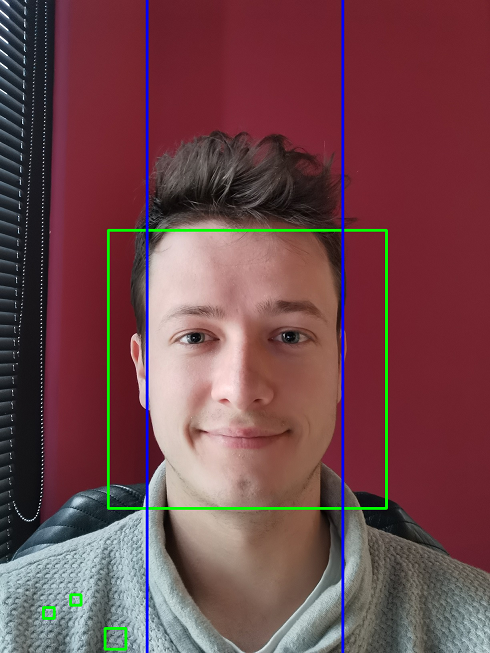
\includegraphics[scale=0.3]{images/face_filter_boundary_1.png}}
            \hspace{8mm}
            \subfigure[Po filtrowaniu. Błędne obszary odrzucone]{\label{fig:face_boundary_after}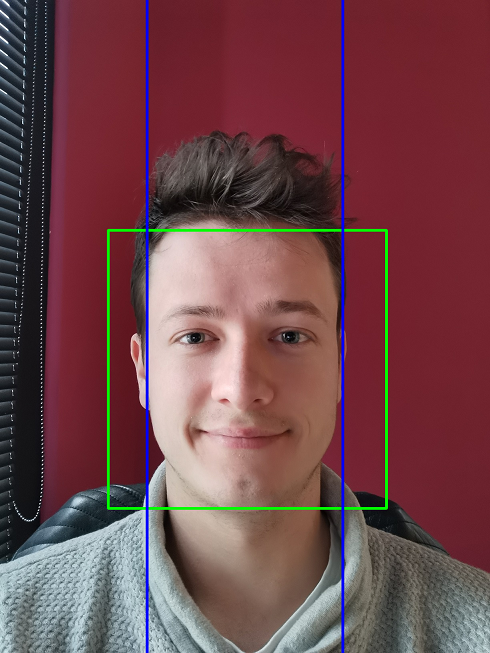
\includegraphics[scale=0.3]{images/face_filter_boundary_2.png}}
        \end{center}
        \caption{Zielone obszary - obszary, w których według klasyfikatora może znajdować się twarz. Niebieskie pasy - obszar, w którym musi znajdować się środek twarzy.}
        \label{fig:face_boundary}
    \end{figure}
    
    \item Kolejnym etapem jest odrzucenie wykrytych obszarów, które wychodzą zbyt daleko za obszar zdjęcia. Jeśli którykolwiek z boków prostokąta wystaje pionowo/poziomo o odleglość większą niż $10\%$ odpowiednio wysokości/szrokości to zostaje odrzucony.
    
    \begin{figure}[H]
        \begin{center}
            \subfigure[Przed filtrowaniem zależnym od wystawania poza obraz. Wykryty dodatkowy błędny obszar]{\label{fig:face_out_before}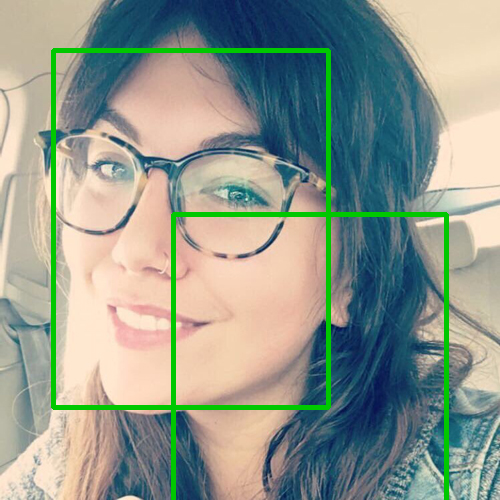
\includegraphics[scale=0.3]{images/face_filter_out_before.png}}
            \hspace{8mm}
            \subfigure[Po filtrowaniu. Błędny obszar odrzucony]{\label{fig:face_out_after}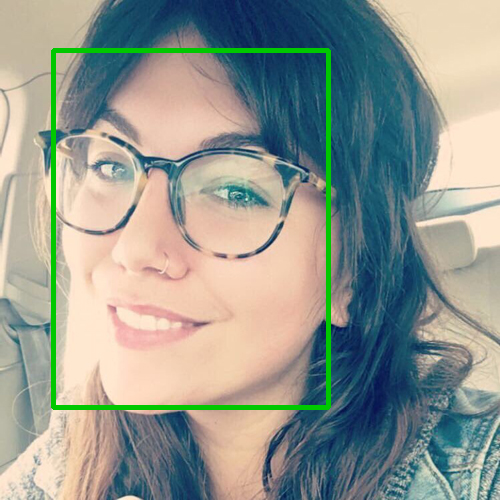
\includegraphics[scale=0.3]{images/face_filter_out_after.png}}
        \end{center}
        \caption{Zielone obszary - obszary, w których według klasyfikatora może znajdować się twarz. Niebieskie pasy - obszar, w którym musi znajdować się środek twarzy.}
        \label{fig:face_out}
    \end{figure}
    
    \item Z pozostałych obszarów wybieram ten, który zajmuje największą powierzechnię. Taki wybór motywuję tym, że twarz użytkownika telefonu na obrazie z kamery przedniej zajmuję większą część płaszczyzny, ponieważ korzystając z urządzenia nie trzymamy go bardzo daleko od siebie oraz własnymi obserwacjami zachowania algorytmów wykrywania twarzy.
    
    \begin{figure}[H]
        \begin{center}
            \subfigure[Przed filtrowaniem zależnym od wielkości. Wykryty dodatkowy błędny obszar]{\label{fig:face_size_before}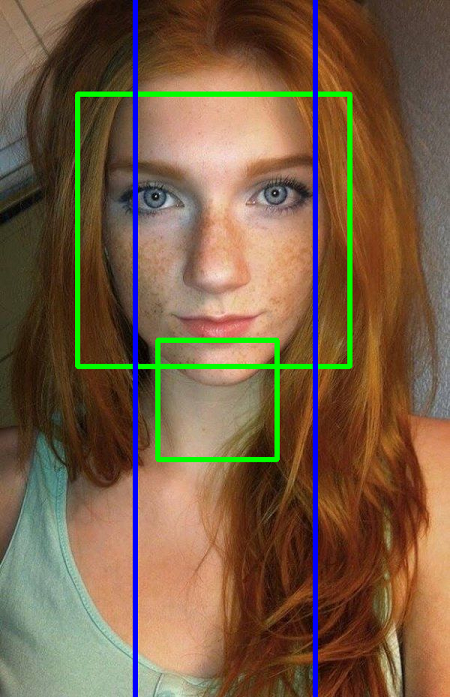
\includegraphics[scale=0.3]{images/face_filter_size_1.png}}
            \hspace{8mm}
            \subfigure[Po filtrowaniu. Błędny obszary odrzucony]{\label{fig:face_size_after}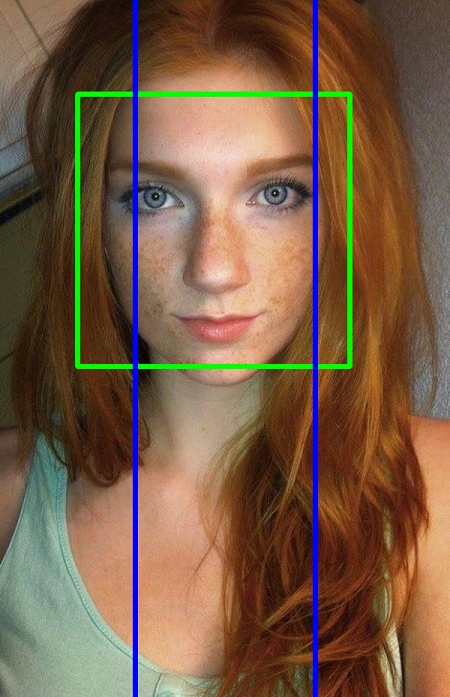
\includegraphics[scale=0.3]{images/face_filter_size_2.png}}
        \end{center}
        \caption{Kilka wykrytych obszarów w środokowej części. Wybieram najwiękzszy. \cite{readheadPortrait1}}
        \label{fig:face_size}
    \end{figure}
    
    
    
\end{itemize}


\section{Porównanie algorytmów detekcji twarzy}

\subsection{Testowanie na statycznych zdjęciach}

Pierwszy etap testowania algorytmów detekcji twarzy będzie bazował na statycznych zdjęciach z datasetu (Patrz rozdz. \hyperref[section:dataset]{\textit{\ref{section:dataset}.Dataset}}). Pozwoli to przetestować na jednakowych danych wszystkie metody pod względem ich skuteczności wykrywania docelowych obszarów w różnych warunkwach oraz uzyskać miarodajne wyniki.

\subsubsection{Oczekiwany wynik}

Każde zdjęcie z datasetu do tego etapu zostało opisane przez dwa prostokąty między którymi powinien znaleźć się wykryta przez algorytm twarz. Obszar ten został dobrany w następujący sposó:

\begin{itemize}
    \item Wewnętrzna część obejmuje minimalny obszar, na którym znajdują się brwi, oczy, nos i usta.
    \item W zewnętrznym prostokącie powinna znaleźć się cała twarz. Powiększony jest o pewną tolerancję. 
\end{itemize}

\begin{figure}[H]
    \begin{center}
        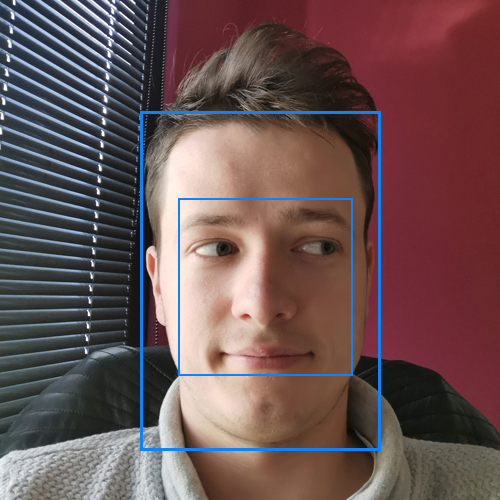
\includegraphics[scale=0.3]{images/face_test_expected.jpg}
        \caption{Oczekiwany obszar detekcji twarzy. }
        \label{fig:face_test_expected}
    \end{center}
\end{figure}

\subsubsection{Sposób testowania}

Dla każdego algorytmu zostanie przeprowadzone testy na zestawach obrazów o następujących właściwościach:

\begin{itemize}
    \item 300x300 RGB
    \item 500x500 RGB
    \item 300x300 skala szarości
    \item 500x500 skala szarości
\end{itemize}

W przypadku DNN Caffe nie jest możliwe przeprowadzenie badań dla zdjęć w skali szarości, ponieważ wymaga on obrazu z trzema kanałami barw.

\subsubsection{Zbierane dane}

Dla każdego rodzaju testu i algorytmu zostaną zebrane następujące dane:

\begin{itemize}
    \item \textbf{Prawidłowe detekcje} - suma perfekcyjnych i częściowo dobrych detekcji
    \item \textbf{Perfekcyjne detekcje} - jeśli wykryty obszar w pełni znajduje się pomiędzy oczekiwanym prostokątami
    \item \textbf{Częściowo dobre detekcje} - jeśli są krawędzie, które znajdują się poza oczekiwanym obszarem, ale w zadowalającej odległości (Patrz uwaga niżej)
    \item \textbf{Z 3 na 4 krawędzie perfekcyjne detekcje} - jeśli tylko jedna krawędź znajduje się poza oczekiwanym obszarem w zadowalającej odległości (Patrz uwaga niżej)
    \item \textbf{Złe detekcje} - jeśli twarz nie została wykryta lub wskazany obszar jest niezadowalający
    \item \textbf{Twarze niewykryte} - jeśli całkowicie nie udało się wykryć twarzy
    \item \textbf{Średnia procentowa odległość błędnych krawędzie} - wyrażony w procentach średni stosunek odległości krawędzi do szerkości/wysokości maskymalnego dopuszczalnego obszaru dla błędnie wykrytych stron
    \item \textbf{Średni czas przetwarzania jednego zdjęcia}
\end{itemize}

\textit{Uwaga 1.} Obszar uznany jest za częściowo dobry jeśli żadna krawędź nie jest oddalona o więcej niż $1.2 x$ i maksymalnie jedna oddalona jest o długość z przedziału $[1.1x, 1.2x]$. Odległość $x$ to szerokość lub wysokość (zależnie od krawędzie) maksymalnego oczekiwanego obszaru twarzy.
\par
\textit{Uwaga 2.} Obszar zaliczony jest do grupy 3/4 perfekcyjnych detekcji, jeśli 3 krawędzie znajdują się w oczekiwanym obszarze, a czwarta odchylona od normy w przedziale $[1.0x, 1.2x]$.
\par 
\textit{Uwaga 3.} Dodatkowy podział złej detekcji na niewykryte twarze wynika z faktu, że metody oparte o Cascasding Classifier na wyjściu podają obszar kwadratowy i przy rozciągniętej lub pochylonej twarzy boczne obszary mogą być bardzo oddalone od oczkiwanej wartości, ale dalej wykryć twarz. 
\par
\textit{Uwaga 4.} Celem miarodajnego wyniku czasu przetwarzania każdy test zostanie przeprowadzony 20 razy, a wyniki uśrednione.

\subsubsection{Wyniki}
\label{section:face_main_test}

% Please add the following required packages to your document preamble:
% \usepackage{graphicx}
% \usepackage[table,xcdraw]{xcolor}
% If you use beamer only pass "xcolor=table" option, i.e. \documentclass[xcolor=table]{beamer}
\begin{table}[H]
\centering
\resizebox{\textwidth}{!}{%
\begin{tabular}{|ccccccccc|}
\hline
 &
  \textbf{\begin{tabular}[c]{@{}c@{}}Prawidłowa\\ detekcja\end{tabular}} &
  \textbf{\begin{tabular}[c]{@{}c@{}}Perfekcyjna\\ detekcja\end{tabular}} &
  \textbf{\begin{tabular}[c]{@{}c@{}}Częściowa\\ dobra\\ detekcja\end{tabular}} &
  \textbf{\begin{tabular}[c]{@{}c@{}}3/4\\ krawędzie\\ perfekcyjne\end{tabular}} &
  \textbf{\begin{tabular}[c]{@{}c@{}}Zła\\ detekcja\end{tabular}} &
  \textbf{\begin{tabular}[c]{@{}c@{}}Niewykryte\\ twarze\end{tabular}} &
  \textbf{\begin{tabular}[c]{@{}c@{}}Średnia\\ odległość\\ złych\end{tabular}} &
  \textbf{\begin{tabular}[c]{@{}c@{}}Średni czas \\ przetwarzania\\ pojedynczego\\ zdjęcia\end{tabular}} \\ \hline
\textbf{Haar Cascade 500x500} &
  69 &
  4 &
  65 &
  32 &
  11 &
  9 &
  6,07 \% &
  0,072 s \\
  
\rowcolor[HTML]{C0C0C0} 
\textbf{Haar Cascade 300x300} &
 68 &
  5 &
  63 &
  33 &
  12 &
   9 &
  6,29 \% &
  0,028 s \\
  
  \textbf{LBP Cascade 500x500} &
  58 &
  4 &
  54 &
  29 &
  22 &
  22 &
  6,22\% &
  0,039 s \\
  
\rowcolor[HTML]{C0C0C0} 
  \textbf{LBP Cascade 300x300} &
  61 &
  4 &
  57 &
  34 &
  19 &
  17 &
  6,29 \% &
  0,014 s \\
  
\textbf{DNN Caffe 500x500} &
  80 &
  68 &
  12 &
  11 &
  0 &
  0 &
  5,49 \% &
  0,079 s \\
  
\rowcolor[HTML]{C0C0C0} 
\textbf{DNN Caffe 300x300} &
  80 &
  62 &
  18 &
  18 &
  0 &
  0 &
  4,87 \% &
  0,073 s \\ 
  
  \hline
\end{tabular}%
}
\caption{Wynik porównania algorytmów detekcji twarzy dla obrazów RGB}
\label{tab:face_detect_result_RGB}
\end{table}

% Please add the following required packages to your document preamble:
% \usepackage{graphicx}
% \usepackage[table,xcdraw]{xcolor}
% If you use beamer only pass "xcolor=table" option, i.e. \documentclass[xcolor=table]{beamer}
\begin{table}[H]
\centering
\resizebox{\textwidth}{!}{%
\begin{tabular}{|ccccccccc|}
\hline
{\color[HTML]{000000} \textbf{}} &
  {\color[HTML]{000000} \textbf{\begin{tabular}[c]{@{}c@{}}Prawidłowa\\ detekcja\end{tabular}}} &
  {\color[HTML]{000000} \textbf{\begin{tabular}[c]{@{}c@{}}Perfekcyjna\\ detekcja\end{tabular}}} &
  {\color[HTML]{000000} \textbf{\begin{tabular}[c]{@{}c@{}}Częściowa\\ dobra\\ detekcja\end{tabular}}} &
  {\color[HTML]{000000} \textbf{\begin{tabular}[c]{@{}c@{}}3/4\\ krawędzie\\ perfekcyjne\end{tabular}}} &
  {\color[HTML]{000000} \textbf{\begin{tabular}[c]{@{}c@{}}Zła\\ detekcja\end{tabular}}} &
  {\color[HTML]{000000} \textbf{\begin{tabular}[c]{@{}c@{}}Niewykryte\\ twarze\end{tabular}}} &
  {\color[HTML]{000000} \textbf{\begin{tabular}[c]{@{}c@{}}Średnia\\ odległość\\ złych\end{tabular}}} &
  {\color[HTML]{000000} \textbf{\begin{tabular}[c]{@{}c@{}}Średni czas \\ przetwarzania\\ pojedynczego\\ zdjęcia\end{tabular}}} \\ \hline
\textbf{Haar Cascade 500x500} &
  69 &
  4 &
  65 &
  31 &
  11 &
  9 &
  6,40 \% &
  0,073 s \\
\rowcolor[HTML]{C0C0C0} 
\textbf{Haar Cascade 300x300} &
  67 &
  4 &
  63 &
  34 &
  13 &
  9 &
  6,43 \% &
  0,028 s \\
  
\textbf{LBP Cascade 500x500} &
  60 &
  5 &
  55 &
  30 &
  20 &
  17 &
  6,17 \% &
  0,038 s \\
  
\rowcolor[HTML]{C0C0C0} 
\textbf{LBP Cascade 300x300} &
  60 &
  4 &
  56 &
  31 &
  20 &
  17 &
  6,65 \% &
  0,013 s \\
  
\textbf{DNN Caffe 500x500} &
  nd. &
  nd. &
  nd. &
  nd. &
  nd. &
  nd. &
  nd. &
  nd. \\
  
\rowcolor[HTML]{C0C0C0} 
\textbf{DNN Caffe 300x300} &
  nd. &
  nd. &
  nd. &
  nd. &
  nd. &
  nd. &
  nd. &
  nd. \\
  
  \hline
\end{tabular}%
}
\begin{center}
    \caption{Wynik porównania algorytmów detekcji twarzy dla obrazów w skali szarości}
\end{center}

\label{tab:face_detect_result_GRAY}
\end{table}


Metoda \textit{Haar Cascade} daje średnio $~69/80$ $(86\%)$ dobrych detekcji. Jest to dosyć przeciętny wynik. Na taki rezultat składa się kilka problemów tej metody. Nie radzi sobie ona dobrze z częściowo zakrytymi twarzami lub gdy głowa jest pochylona w bok. Nie wykrywa w ogóle twarzy jeśli zdjęcie jest zbyt jasne, twarz oświetlona lub źródło światła świeci prosto w obiektyw. Na plus tej metody można zapisać małą ilość zwróconych przez nią dodatkowych, błędnych obszarów, które musiały zostać odfiltorwane.

\par
\textit{Cascading Classifier} bazując na modelu \textit{LBP} miał najgorsze wyniki detekcji twarzy - na poziomie $~60/80$ $(75 \%)$. Jednak co zwraca uwagę to fakt, że bardzo duży odsetek twarzy nie zoystał w ogóle wykryty. Występują tu te same problemy co w \textit{Haar Cascade}, ale dodatkowo algorytm nie radzi sobie gdy twarz zajmuje prawie całe zdjęcie.

\par
Najlepszy wynik detekcji uzyskał bezdyskusyjnie \textit{DNN Caffe}. Fakt, że w każdym z dwóch testów wykrył on $100 \%$ twarzy robi wrażenie. Co więcej perfekcyjne detekcje były na poziomie $~65/80$ $(81,25 \%)$. Nie występują tu problemy takie jak w poprzednich algorytmach. Radzi sobie on dobrze w złych warunkach oświetleniowych. Częsciowe zakrycie twarzy nie wpływa na detekcję. Wykrywa on dobrze zarówno pochyolne jak i odwrócone twarze. Jedyną negatywnym zjawiskiem, które zaobserwowałem w tej metodzie to zwracanie wielu dodatkowych obszarów, które są błędne. Zastosowanie filtrowania pozwoliło jednak odrzucić wszystkie błędne obszary.

\vspace{5mm}
Różnica w procencie perfekcyjnych detekcji pomiędzy \textit{DNN Caffe}, a \textit{LBP} i \textit{Haar} wynika z rodzaju obszaru zwracanym przez te algorytmy. Metoda oparta na głębokich sieciach neuronowych zwraca prostokąt o dowolnym stosunku boków, natomiast druga grupa zwraca kwadrat. Dzięki temu \textit{DNN} lepiej dopasowuję się do kształtu twarzy niż \textit{Cascading Classifier}.

\vspace{5mm}

Najszbyszy okazał się algorytm operujący na modelu \textit{LBP}. \textit{DNN Caffe} dla zdjęć $500x500$  był porównywalnie szybki jak \textit{Haar Cascade}, natomiast już w przypadku $300x300$ około $2.5$ razy wolniejszy.
\par
Co ciekawe i warte odnotowania to fakt, że algorytm \textit{DNN} przetwarzał prawie tak samo szybko obie rozdzielczości zdjęć. Można wysnuć tezę, że dla tej metody wielkość obrazu nie ma wpływu na szybkość przetwarzania. Ze względu, że taka właściwość może okazać się przydatna w perspektywie dalszych etapów projektu, zamierzam zbadać tę zależność w następnym rozdziale.

\vspace{5mm}

Zmiana detekcji z trójkanałowej RGB na skale szarości nie przyniosło żadnej zmiany zarówno w skuteczności algorytmów, jak również nie skróciło czasu detekcji.

\subsection{Dodatkowe testy \textit{DNN Caffe}}

\subsubsection{Wpływ wielkości zdjęcia na czas przetwarzania}

% Please add the following required packages to your document preamble:
% \usepackage{graphicx}
% \usepackage[table,xcdraw]{xcolor}
% If you use beamer only pass "xcolor=table" option, i.e. \documentclass[xcolor=table]{beamer}
\begin{table}[H]
\centering
\resizebox{\textwidth}{!}{%
\begin{tabular}{|ccccccccc|}
\hline
 &
  \textbf{\begin{tabular}[c]{@{}c@{}}Prawidłowa\\ detekcja\end{tabular}} &
  \textbf{\begin{tabular}[c]{@{}c@{}}Perfekcyjna\\ detekcja\end{tabular}} &
  \textbf{\begin{tabular}[c]{@{}c@{}}Częściowa\\ dobra\\ detekcja\end{tabular}} &
  \textbf{\begin{tabular}[c]{@{}c@{}}3/4\\ krawędzie\\ perfekcyjne\end{tabular}} &
  \textbf{\begin{tabular}[c]{@{}c@{}}Zła\\ detekcja\end{tabular}} &
  \textbf{\begin{tabular}[c]{@{}c@{}}Niewykryte\\ twarze\end{tabular}} &
  \textbf{\begin{tabular}[c]{@{}c@{}}Średnia\\ odległość\\ złych\end{tabular}} &
  \textbf{\begin{tabular}[c]{@{}c@{}}Średni czas \\ przetwarzania\\ pojedynczego\\ zdjęcia\end{tabular}} \\ \hline
\textbf{300x300} &
  80 &
  62 &
  18 &
  18 &
  0 &
  0 &
  4,87 \% &
  0,064 s \\
  
\rowcolor[HTML]{C0C0C0} 
\textbf{500x500} &
  80 &
  68 &
  12 &
  11 &
  0 &
  0 &
  5,49 \% &
  0,065 s \\
  
\textbf{1000x1000} &
  80 &
  67 &
  13 &
  13 &
  0 &
  0 &
  5,31 \% \% &
  0,066 s \\
  
\rowcolor[HTML]{C0C0C0} 
  \textbf{2000x2000} &
  80 &
  65 &
  15 &
  15 &
  0 &
  0 &
  4,62 \% &
  0,062 s \\
 
  \hline
\end{tabular}%
}
\caption{Wpływ rozdzielczości zdjęcia na detekcję DNN}
\label{tab:face_dnn_speed}
\end{table}

Test ten potwierdza postawioną przeze mnie wcześniej tezę, że wielkość zdjęcia nie ma wpływu na szybkość przetwarzania algorytmu \textit{DNN Caffe}. Testy w każdej rozdzielczości zostały wykonane mniej więcej w tym samym czasie, a rożnica zapewne wynika z urządzenia w różnych chwilach i jest pomijalna.

\textit{Uwaga}. Różncia czasów DNN między tym testem, a \hyperref[{section:face_main_test}]{\textit{poprzednim}} prawdopodobnie wynika z jakichś obciążeń telefonu w danym momencie.

\subsubsection{Porównanie precyzji detekcji zależnie od sposóbu filtrowania}

Metoda oparta na głębokich sieciach neuronowych na wyjściu zwraca wiele obszarów wraz z wksaźnikiem pewności detekcji. Im większy współczynnik tym w teorii większa szansa, że jest to objekt, który chcieliśmy wykryć.
\par
Z tego powodu postanowiłem porównać autorskie filtrowanie opisane wcześniej (patrz rozdz. \hyperref[{section:face_detection_filter}]{\textit{\ref{section:face_detection_filter}.Filtrowanie wyników}}) i wybór detekcji z największym procentem pewności.

% Please add the following required packages to your document preamble:
% \usepackage{graphicx}
% \usepackage[table,xcdraw]{xcolor}
% If you use beamer only pass "xcolor=table" option, i.e. \documentclass[xcolor=table]{beamer}
\begin{table}[H]
\centering
\resizebox{\textwidth}{!}{%
\begin{tabular}{|ccccccccc|}
\hline
 &
  \textbf{\begin{tabular}[c]{@{}c@{}}Prawidłowa\\ detekcja\end{tabular}} &
  \textbf{\begin{tabular}[c]{@{}c@{}}Perfekcyjna\\ detekcja\end{tabular}} &
  \textbf{\begin{tabular}[c]{@{}c@{}}Częściowa\\ dobra\\ detekcja\end{tabular}} &
  \textbf{\begin{tabular}[c]{@{}c@{}}3/4\\ krawędzie\\ perfekcyjne\end{tabular}} &
  \textbf{\begin{tabular}[c]{@{}c@{}}Zła\\ detekcja\end{tabular}} &
  \textbf{\begin{tabular}[c]{@{}c@{}}Niewykryte\\ twarze\end{tabular}} &
  \textbf{\begin{tabular}[c]{@{}c@{}}Średnia\\ odległość\\ złych\end{tabular}} &
  \textbf{\begin{tabular}[c]{@{}c@{}}Średni czas \\ przetwarzania\\ pojedynczego\\ zdjęcia\end{tabular}} \\ \hline
\textbf{Autorskie filtrowanie 300x300} &
  80 &
  62 &
  18 &
  18 &
  0 &
  0 &
  4,87 \% &
  0,069 s \\
  
\rowcolor[HTML]{C0C0C0} 
\textbf{Autorskie filtrowanie  500x500} &
  80 &
  68 &
  12 &
  11 &
  0 &
  0 &
  5,49 \% &
  0,072 s \\
  
\textbf{Najwyższy współczynnik pewności 300x300} &
  76 &
  58 &
  18 &
  18 &
  4 &
  4 &
  4,87 \% \% &
  0,064 s \\
  
\rowcolor[HTML]{C0C0C0} 
  \textbf{Najwyższy współczynnik pewności 500x500} &
  76 &
  64 &
  12 &
  11 &
  4 &
  4 &
  5,49 \% &
  0,068 s \\
 
  \hline
\end{tabular}%
}
\caption{Wynik porównania sposobów filtrowania detekcji}
\label{tab:face_filter_test}
\end{table}

Jak widać zaproponowana przeze mnie wcześniej sekwencja filtrowania wykrytych obszarów daje lepsze rezultaty niż wybór najwyższego współczynnika pewności.

\_\_\_\_\_\_ TODO \_\_\_\_\_\_ 



\subsection{Testowanie na obrazie z kamery na żywo}



\section{Detekcja oczu}

Przed przystąpieniem do detekcji oczu należy wyznaczyć obszar, na którym wykryta została twarz. Następnie obcinając klatkę tylko do ustalonego prostokąta wykrywam oczy za pomocą Cascading Classifier - podobnie jak twarz.

Wynik który chcę uzyskać - wykryte oczy powinny się znaleźć pomiędzy naniesionymi prostkątami:

\begin{figure}[H]
    \begin{center}
        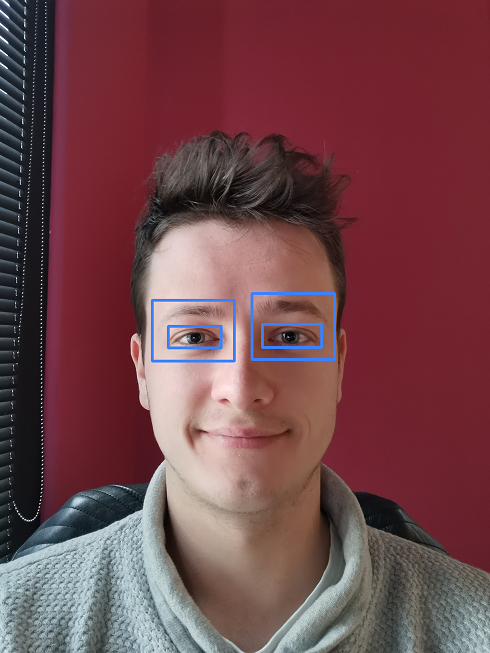
\includegraphics[scale=0.6]{images/expected_eyes_region.png}
        \caption{Przybliżony obszar oczu, który chcę wykrywać}
        \label{fig:expected_eyes_region}
    \end{center}
\end{figure}

\subsection{Obcięcie obszaru detekcji}
Dodatkowo - prócz detekcji jedynie na obszarze twarzy - zdecydowałem się zawęźić płaszczyznę przeszukiwań.
Wstępnie metodą prób i błędów dobrałem następujące parametry obcięcia obszaru:
\begin{itemize}
    \item Góra: $0.1$
    \item Dół: $0.45$
    \item Lewo: $0.1$
    \item Prawo: $0.1$
\end{itemize}

Parametr określa jaka część obszaru zostaje pominięta z poszczególnych stron.

\begin{figure}[H]
    \begin{center}
        \subfigure[Wykryty obszar twarzy]{\label{fig:eye_crop_before}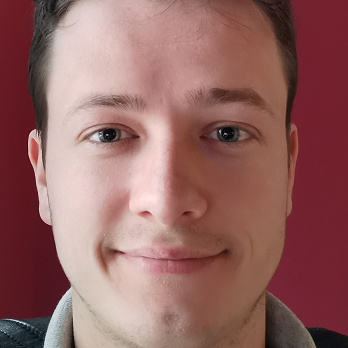
\includegraphics[scale=0.6]{images/eye_cropped_face.png}}
        \hspace{8mm}
        \subfigure[Wycięty obszar oczu]{\label{fig:eye_crop_after}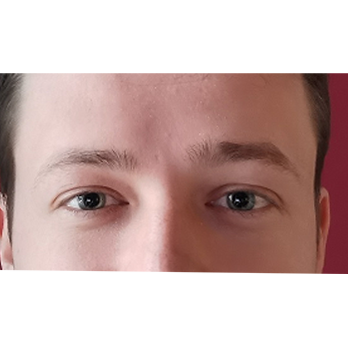
\includegraphics[scale=0.6]{images/eye_cropped_eyes.png}}
    \end{center}
    \caption{Obcięcie obszaru detekcji oczu}
    \label{fig:eye_crop}
\end{figure}

Takie zawężenie obszaru detekcji pozwoliło wyliminować cześć z błędnie oznaczonych oczu - poniżej środka twarzy czy w bok od rzeczywistego położenia:

\begin{figure}[H]
    \begin{center}
        \subfigure[Wykrywanie oczu bez dodatkowego obcięcia obszaru]{\label{fig:eye_detect_crop_before}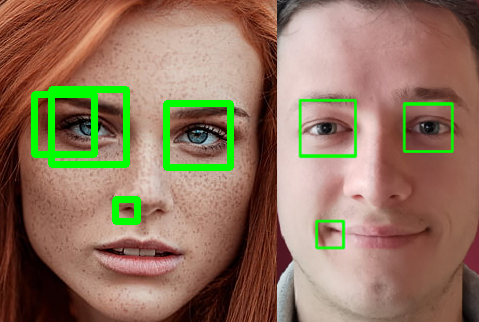
\includegraphics[scale=0.45]{images/eye_detect_before_crop_1.png}}
        \hspace{8mm}
        \subfigure[Wykrywanie oczu z dodatkowym obcięciem obszaru]{\label{fig:eye_detect_crop_after}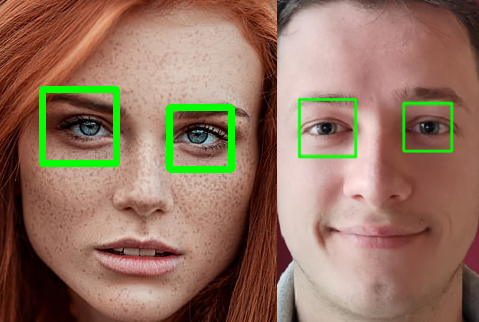
\includegraphics[scale=0.45]{images/eye_detect_after_crop_1.png}}
    \end{center}
    \caption{Poprawienie rezultatu detekcji oczu po dodatkowym obcięciu obszaru. \cite{readheadPortrait2}}
    \label{fig:eye_detect_crop}
\end{figure}

{\_\_\_\_} przyszłości zrobić testy na wielu zdjęciach wraz z wynikami przed/po w formie liczbowej. {\_\_\_\_}

\subsection{Filtrowanie wyników}

Ze względu na możliwość błędnych wskazań wprowadziłem filtrowanie wyników detekcji oczu. \\
Algorytm filtrowania składa się z dwóch etapów:

\begin{itemize}
    \item Podzielenie wykrytych obszarów na dwie grupy - na lewą i prawą stronę twarzy
    \item W obu grup wybranie największego obszaru
\end{itemize}

Dodatkowo pozwoliło to na łatwe zidentyfikowanie który obszar to które oko i ich posportowanie.

\begin{figure}[H]
    \begin{center}
        \subfigure[Detekcja oczu z błędnymi obszarami]{\label{fig:eye_filter_before}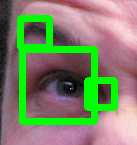
\includegraphics[scale=1.0]{images/eye_filter_before.png}}
        \hspace{8mm}
        \subfigure[Przefiltrowane obszary detekcji oczu]{\label{fig:eye_filter_after}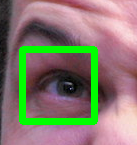
\includegraphics[scale=1.0]{images/eye_filter_after.png}}
    \end{center}
    \caption{Efekt filtrowania obszarów detekcji oczu}
    \label{fig:eye_filter}
\end{figure}


\section{Detekcja źrenic}

Do wykrywania źrenic, najpierw musimy wyznaczyć obszar oczu. Następnie korzystając z jednych z poniższch metod ustalam interesujący nas środek. \\
Wynik, który w przybliżeniu chcę uzyskać:

\begin{figure}[H]
    \begin{center}
        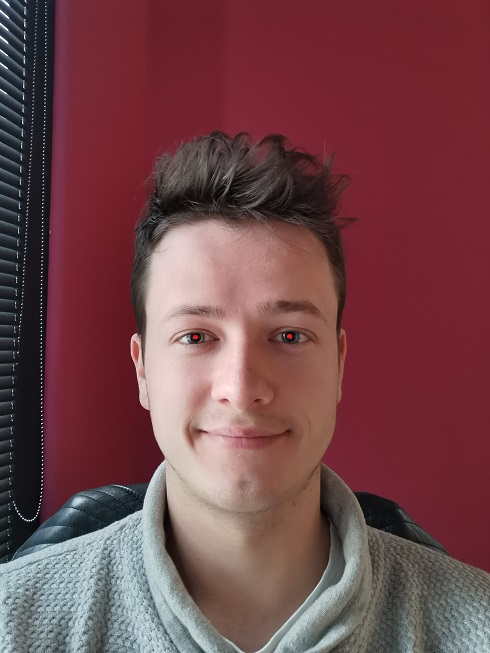
\includegraphics[scale=0.35]{images/expected_pupils.jpg}
        \caption{W przybliżeniu środek źrenic, który chcę uzyskać}
        \label{fig:expected_pupils}
    \end{center}
\end{figure}

\subsection{Algorytm CDF}
Algorytm zaimplementowany na podstawie dwóch artykułów o detekcji źrenic \cite{IMECSPupilCDFAnalysis}
\cite{EyePupilWebCam}. Opiera się w głównej mierze na progowaniu za pomocą dystrybuanty. Cały algorytm przetwarza obszar oka w skali szarości. \\
Metoda ta daje całkiem dobre i prawdopodobnie wystarczające rezultaty. \\

\begin{figure}[H]
    \begin{center}
        \subfigure[Oko skierowane w prawo]{\label{fig:pupil_cdf_left}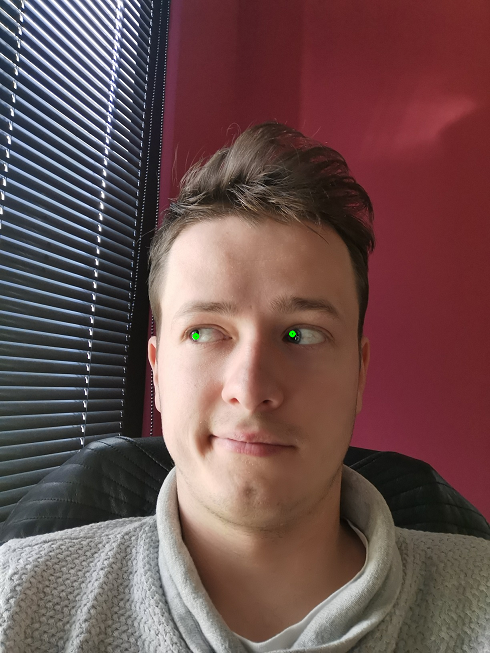
\includegraphics[scale=0.3]{images/pupil_2eyes_left_1.png}}
        \hspace{3mm}
        \subfigure[Oko skierowane na wprost]{\label{fig:pupil_cdf_center}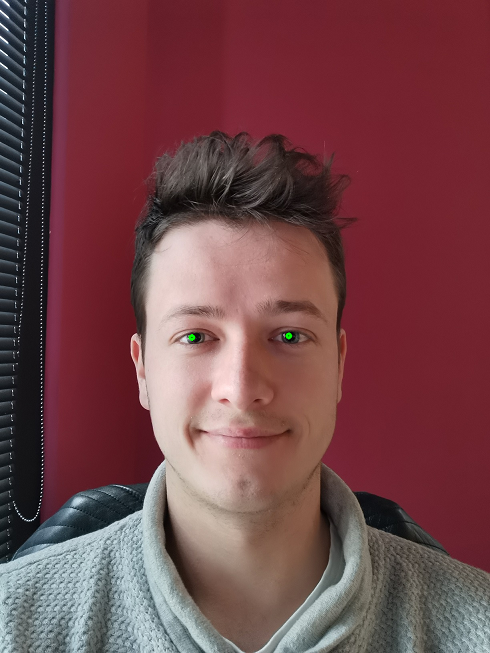
\includegraphics[scale=0.3]{images/pupil_2eyes_center_1.png}}
        \hspace{3mm}
        \subfigure[Oko skierowane w lewo]{\label{fig:pupil_cdf_right}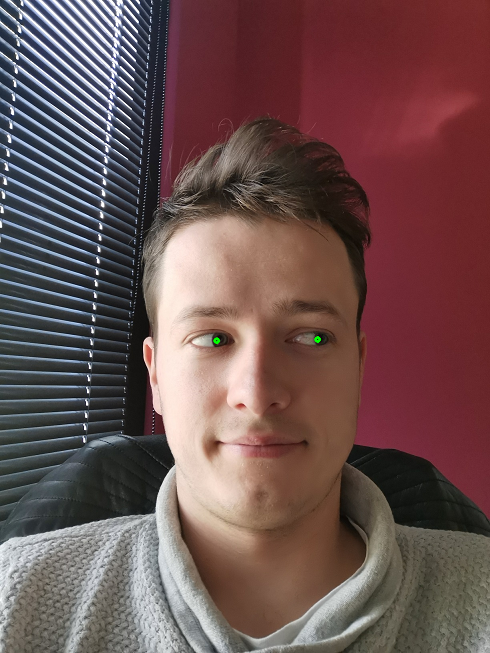
\includegraphics[scale=0.3]{images/pupil_2eyes_right_1.png}}
    \end{center}
    \caption{Rezultat wykrywania źrenic metodą CDF}
    \label{fig:cdf_results}
\end{figure}

\subsubsection{Kroki algorytmu}

\begin{itemize}
    \item Za pomocą progowania z użyciem dystrybuanty CDF tworzymy obraz binarny\\
    \begin{equation}
        CDF(r) = \sum_{w=0}^{r} p(w)
    \end{equation}
    Gdzie \textit{p(w)} to prawdopodobieństwo znalezienia punktu o jasności równej \textit{w} - określone przy pomocy dystrybuanty dystrybuanty.
    
    \begin{equation}
        I`(x, y) = 
        \begin{cases}
            255, &  CDF(I(x, y)) < \textit{a}\\
            0,   &  wpp
        \end{cases}
    \end{equation} 
    
    Gdzie \textit{I} to jasność piksela, natomiast \textit{a} to ustalony próg

    \item Na uzyskany obraz binarny nakładamy operację morfologiczną erozji (filtr minimalny), celem usunięcia pojedynczych ciemnych pikseli
    
    \item Znajdujemy najciemniejszy piksel na oryginalnym obrazie wśród tych, które mają wartość 255 (są białe) na obrazie binarnym
    
    \item Obliczamy średnią jasność pikseli w kawdracie 10x10 wokół wybranego najciemniejszego punktu
    
    \item Nakładamy erozję na obszarze 15x15 wokół wybranego punktu
    \item Na tym obszarze stosujemy progowanie
    
    \begin{equation}
        I`(x, y) = 
        \begin{cases}
            255, &  I(x, y) < AVG_I\\
            0,   &  wpp
        \end{cases}
    \end{equation}
    
    Gdzie \textit{AVG$_I$} to średnia jasność obszaru obliczona wcześniej
    
    \item Środkiem źrenicy będzie środek ciężkości białych punktów na binarnym obszarze, który uzyskaliśmy

\end{itemize}


\begin{figure}[H]
    \begin{center}
        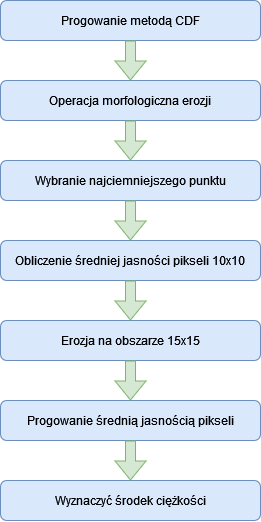
\includegraphics[scale=0.35]{images/CDF_Diagram.png}
        \caption{Kroki algorytmu metodą CDF}
        \label{fig:cdf_diagram}
    \end{center}
\end{figure}

\subsubsection{Wynik kolejnych etapów algorytmu}


\begin{figure}[H]
    \begin{center}
        \subfigure[Obszar oka w RGB]{\label{fig:cdf_rgb}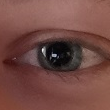
\includegraphics[scale=0.50]{images/CDF_steps/CDF_rgb_eye.png}}
        \hspace{8mm}
        \subfigure[Obszar oka w skali szarości]{\label{fig:cdf_gray}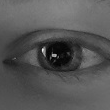
\includegraphics[scale=0.50]{images/CDF_steps/CDF_gray_eye.png}}
        \hspace{8mm}
        \subfigure[Wynik progowania CDF]{\label{fig:cdf_binary}
\includegraphics[scale=0.50]{images/CDF_steps/CDF_binary_eye_after_CDF.png}}
        
        \hfill
        
        \subfigure[Wynik erozji]{\label{fig:cdf_erode}
\includegraphics[scale=0.50]{images/CDF_steps/CDF_binary_eye_after_erode.png}}
        \hspace{8mm}
        \subfigure[Najciemniejszy punkt]{\label{fig:cdf_darkest}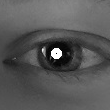
\includegraphics[scale=0.50]{images/CDF_steps/CDF_darkest_pixel.png}}
        \hspace{8mm}
        \subfigure[Obszar 15x15 wokół najciemniejszego punktu ]{\label{fig:cdf_pmi}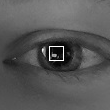
\includegraphics[scale=0.50]{images/CDF_steps/CDF_pmi.png}}
        
        \hfill
        
        \subfigure[Wynik erozji]{\label{fig:cdf_eroded_pmi}
\includegraphics[scale=0.50]{images/CDF_steps/CDF_eroded_pmi.png}}
        \hspace{8mm}
        \subfigure[Progowanie średnią jasnością pikseli]{\label{fig:cdf_threshold}
\includegraphics[scale=0.50]{images/CDF_steps/CDF_threshold_pmi.png}}
        \hspace{8mm}
        \subfigure[Wykryte położenie źrenicy]{\label{fig:cdf_pupil_detected}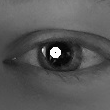
\includegraphics[scale=0.50]{images/CDF_steps/CDF_pupil_detected.png}}
        
    \end{center}
    \caption{Kolejne etapy wykrywania źrenic metodą CDF}
    \label{fig:cdf_steps}
\end{figure}

\subsection{Algorytm PF}
{\_\_\_\_} W przyszłości do testów zaimplementować algorytm PF\cite{EyePupilWebCam} {\_\_\_\_}

\subsection{Algorytm EA}
{\_\_\_\_} W przyszłości do testów zaimplementować algorytm EA\cite{EyePupilWebCam} {\_\_\_\_}

\section{Landmarks}

Są to punkty nakładane na twarz wokół interesujących obszarów - takich jak oczy, nos czy usta. Pozwalają określić położenie, rozmiar czy kształt tych obiektów. Mogą być również użyte do predykcji czy mamy zamknięte/otwarte oczy lub czy się uśmiechamy. 

\subsection{OpenCV-contrib}
Dodatkowe moduł opencv facemark (\textit{OpenCV-contrib}) zawiera trzy algorytmy detekcji landmarków:

\begin{itemize}
    \item Kazemi
    \item AAM
    \item LBF
\end{itemize}

\subsubsection{FacemarkLBF}

Używając metody FacemarkLBF oraz modelu \textit{lbfmodel.yaml} określiłem punkty orientacyjne twarzy. \cite{landmarkSatyaMallick}

\begin{figure}[H]
    \begin{center}
        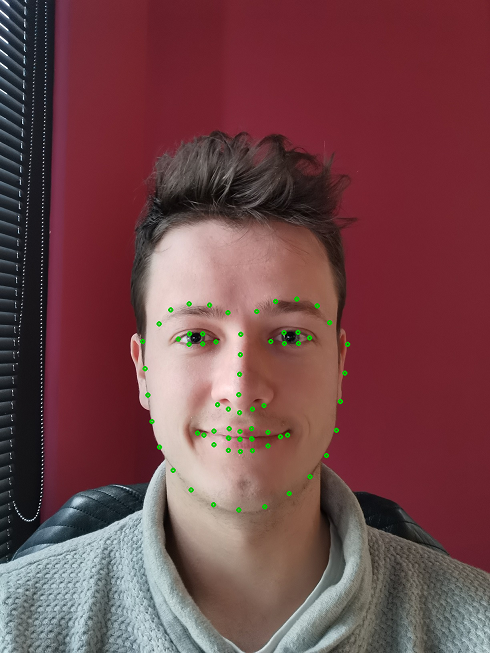
\includegraphics[scale=0.6]{images/landmarks_1.png}
        \caption{Twarz z naniesionymi landmarkami}
        \label{fig:landmarks_1}
    \end{center}
\end{figure}

\section{EAR - Eye Aspect Ratio}
Metoda wykorzystująca landmarki na twarzy. Posiadając oznaczone za pomocą tej metody oczy możemy obliczyć tzw. \textit{EAR}, czyli stosunek otwarcia oczu - wysokość do szerokości widocznej części gałki ocznej. \cite{EARRaspberryPi} \cite{eyeBlinkEARRosebrock}\\

Zależnie od ilości punktów wokół oka będzie różny wzór obliczania EAR.\\
Dla 6 punktów:
\begin{equation}
    EAR = \frac{dist(L_0, L_1) + dist(L_2, L4)}{2 * dist(L_3, L_5)}
\end{equation}
\\
Natomiast, dla 4 punktów:
\begin{equation}
    EAR = \frac{dist(L_0, L_2)}{dist(L_1, L_3)}
\end{equation}

Gdzie \textit{$L_x$} to kolejne landmarki dokoła oczu, a \textit{dist} to odległość między dwoma punktami (odległość euklidesowa).\\

W teorii otwarte oczy będą miały większy wymiar liczbowy EAR, niż oczy zamknięte. Na zdjęciu poniżej widać, że oko otwarte ma większe odległości między punktami pionowymi niż w przypadku  oka zamkniętego. 

\begin{figure}[H]
    \begin{center}
        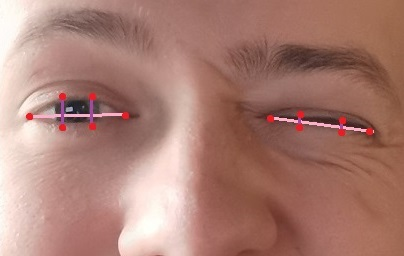
\includegraphics[scale=0.35]{images/theoretical_eye_landmarks.jpg}
        \caption{Teoretyczny rozmieszczene landmarków wokół oczu wraz z naniesionymi połączeniami do obliczenia EAR}
        \label{fig:theoretical_eye_landmarks}
    \end{center}
\end{figure}


\subsection{Testowanie z użyciem landmarków LBF opencv-contrib
}

\subsubsection{Test z użyciem kamery na żywo}

Wykonałem kilka krótkich testów z użyciem obrazu pochodzącego z przedniej kamery telefonu. 
\\
Poniżej znajdują się trzy testy, na których mrugnąłem tylko raz - lewym okiem, prawym i oboma na raz.

\begin{figure}[H]
    \centering
    \begin{tikzpicture}
        \begin{axis}[
            xlabel = {Nr klatki obrazu z kamery},
            ylabel = {EAR},
            height = 0.5\linewidth,
            width = \linewidth,
            ymin= {0.10},
            ymax={0.30},
            ytick = {0.10, 0.12, 0.14, 0.16, 0.18, 0.20, 0.22, 0.24, 0.26, 0.28, 0.30},
            ymajorgrids = {true},
        ]
            \addplot[color=blue, mark=square*] table [x=x, y=a, col sep=comma] {logs/ear_left_1.csv};
            \addplot[color=red, mark=square*] table [x=x, y=b, col sep=comma] {logs/ear_left_1.csv};
        \end{axis}
    \end{tikzpicture}
    \caption{Mrugnięcie lewym okiem}
    \label{fig:left_eye_blink}
\end{figure}


\begin{figure}[H]
    \centering
    \begin{tikzpicture}
        \begin{axis}[
            xlabel = {Nr klatki obrazu z kamery},
            ylabel = {EAR},
            height = 0.5\linewidth,
            width = \linewidth,
            ymin= {0.10},
            ymax={0.30},
            ytick = {0.10, 0.12, 0.14, 0.16, 0.18, 0.20, 0.22, 0.24, 0.26, 0.28, 0.30},
            ymajorgrids = {true},
        ]
            \addplot[color=blue, mark=square*] table [x=x, y=a, col sep=comma] {logs/ear_right_1.csv};
            \addplot[color=red, mark=square*] table [x=x, y=b, col sep=comma] {logs/ear_right_1.csv};
        \end{axis}
    \end{tikzpicture}
    \caption{Mrugnięcie prawym okiem}
    \label{fig:right_eye_blink}
\end{figure}

\begin{figure}[H]
    \centering
    \begin{tikzpicture}
        \begin{axis}[
            xlabel = {Nr klatki obrazu z kamery},
            ylabel = {EAR},
            height = 0.5\linewidth,
            width = \linewidth,
            ymin= {0.10},
            ymax={0.30},
            ytick = {0.10, 0.12, 0.14, 0.16, 0.18, 0.20, 0.22, 0.24, 0.26, 0.28, 0.30},
            ymajorgrids = {true},
        ]
            \addplot[color=blue, mark=square*] table [x=x, y=a, col sep=comma] {logs/ear_both_1.csv};
            \addplot[color=red, mark=square*] table [x=x, y=b, col sep=comma] {logs/ear_both_1.csv};
        \end{axis}
    \end{tikzpicture}
    \caption{Mrugnięcie oboma oczami na raz}
    \label{fig:both_eyes_blink}
\end{figure}


Testy z pojedynczym mruganiem w krótkim okresie czasu dają przyzwoite wyniki i można na nich okreslić moment mrugania. W szczególności przy mrugnięciu jednym okiem.\\

Poniżej rozciągnąłem w czasie test na sekwencje kilku mrugnięć.

\begin{figure}[H]
    \centering
    \begin{tikzpicture}
        \begin{axis}[
            xlabel = {Nr klatki obrazu z kamery},
            ylabel = {EAR},
            height = 0.5\linewidth,
            width = \linewidth,
            ymin= {0.10},
            ymax={0.30},
            ytick = {0.10, 0.12, 0.14, 0.16, 0.18, 0.20, 0.22, 0.24, 0.26, 0.28, 0.30},
            ymajorgrids = {true},
        ]
            \addplot[color=blue, mark=square*] table [x=x, y=a, col sep=comma] {logs/ear_long_1.csv};
            \addplot[color=red, mark=square*] table [x=x, y=b, col sep=comma] {logs/ear_long_1.csv};
        \end{axis}
    \end{tikzpicture}
    \caption{Kilka mrugnięć}
    \label{fig:multi_blinks_1}
\end{figure}

\begin{figure}[H]
    \centering
    \begin{tikzpicture}
        \begin{axis}[
            xlabel = {Nr klatki obrazu z kamery},
            ylabel = {EAR},
            height = 0.5\linewidth,
            width = \linewidth,
            ymin= {0.10},
            ymax={0.30},
            ytick = {0.10, 0.12, 0.14, 0.16, 0.18, 0.20, 0.22, 0.24, 0.26, 0.28, 0.30},
            ymajorgrids = {true},
        ]
            \addplot[color=blue, mark=square*] table [x=x, y=a, col sep=comma] {logs/ear_long_2.csv};
            \addplot[color=red, mark=square*] table [x=x, y=b, col sep=comma] {logs/ear_long_2.csv};
        \end{axis}
    \end{tikzpicture}
    \caption{Kilka mrugnięć}
    \label{fig:multi_blinks_2}
\end{figure}

\begin{figure}[H]
    \centering
    \begin{tikzpicture}
        \begin{axis}[
            xlabel = {Nr klatki obrazu z kamery},
            ylabel = {EAR},
            height = 0.5\linewidth,
            width = \linewidth,
            ymin= {0.10},
            ymax={0.30},
            ytick = {0.10, 0.12, 0.14, 0.16, 0.18, 0.20, 0.22, 0.24, 0.26, 0.28, 0.30},
            ymajorgrids = {true},
        ]
            \addplot[color=blue, mark=square*] table [x=x, y=a, col sep=comma] {logs/ear_long_3.csv};
            \addplot[color=red, mark=square*] table [x=x, y=b, col sep=comma] {logs/ear_long_3.csv};
        \end{axis}
    \end{tikzpicture}
    \caption{Kilka mrugnięć}
    \label{fig:multi_blinks_3}
\end{figure}

Tu również z dużym prawdopodobieństwem można okreśilć, w których klatkach wystąpiło mrugnięcie - widać gwałtowne obniżenie wartości EAR.
\\
Najlepsze wyniki były w przypadku pierwszego testu, ponieważ widać wtedy znaczną różnicę EAR między otwartym ($\sim0.26 - 0.30$), a zamkniętym okiem ($\sim0.12-0.18$). Na pozostałych testach różnice nie były już tak znaczące - na ostatnich dwóch wykresach otwarte i zamknięte oko ma niewielką różnicę w EAR. Takie małe różnice wyników mogą uniemożliwić prawidłową detekcję.

\vspace{3mm}
W każdym z przypadków testowych EAR dla jednego i drugiego oka prawie się pokrywają. Nawet przy mruganiu tylko jednym. Nie pozwoli to więc okręślić, którym okiem użytkownik mrugał.

\vspace{3mm}

Niewątpliwą trudnością w przypadku tej metody byłoby określenie progu wartości EAR, które zakwalifikowałbym jako mrugnięcie. Patrząc na wykresy powyżej można by przyjąć, że jest to wartość koło $~0.18$. Jednak w przypadku ostatecznego wyboru tej metody wymagałoby to dodatkowych badań celem określenia tej wartości.


\subsubsection{Niedokładność nakładania landmarków}

Patrząc jednak na położenie tych landmarków wokół oczu mam wątpliwości co do skuteczności tej metody:

\begin{figure}[H]
    \begin{center}
        \subfigure[]{\label{fig:landmarks_accuracy_1}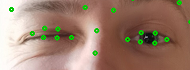
\includegraphics[scale=1.6]{images/landmarks_accuracy_1.png}}
        \hspace{8mm}
        \subfigure[]{\label{fig:landmarks_accuracy_2}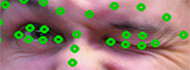
\includegraphics[scale=1.6]{images/landmarks_accuracy_2.png}}
    \end{center}
    \caption{Landmarki na oczach otwartych/zamkniętych}
    \label{fig:landmarks_accuracy_}
\end{figure}

Jak widać algorytm całkiem dobrze radzi sobie z rozmieszczeniem landmarków w przypadku otwartych oczu. Natomiast gdy oczy są zamknięte widać dużą niedokładność, która na pewno w dużym stopniu utrudnia prawidłową detekcję mrugnięcia.

\printbibliography

\end{document}
